% Created 2021-09-04 Sat 15:34
% Intended LaTeX compiler: pdflatex
\documentclass[11pt]{article}
\usepackage[hyphens]{url}
\usepackage{float}
\usepackage[utf8]{inputenc}
\usepackage[T1]{fontenc}
\usepackage{graphicx}
\usepackage{grffile}
\usepackage{longtable}
\usepackage{wrapfig}
\usepackage{rotating}
\usepackage[normalem]{ulem}
\usepackage{amsmath}
\usepackage{textcomp}
\usepackage{amssymb}
\usepackage{capt-of}
\usepackage{hyperref}
\author{Tigany Zarrouk}
\date{\today}
\title{Pure Ti fitting}
\hypersetup{
 pdfauthor={Tigany Zarrouk},
 pdftitle={Pure Ti fitting},
 pdfkeywords={},
 pdfsubject={},
 pdfcreator={Emacs 27.2 (Org mode 9.4)}, 
 pdflang={English}}
\begin{document}

\maketitle
\tableofcontents


\section{Fitting a titanium tight-binding model}
\label{sec:org41025e0}
\label{ch:ti_fitting}
\subsection{Introduction (What, how, where, when, why?)}
\label{sec:orge068ceb}
Fitted canonical d titanium model such that we could have a better
description of titanium within a tight-binding framework. Empirical
potential are not accurate enough to describe the intricacies of the
titanium structure.

\subsection{Fitting}
\label{sec:org711ffe9}

The overlap integrals were chosen to have a simple exponential
distance dependence, as initially formulated by Ducastelle,
\cite{Ducastelle1970c} and Allan \cite{Allan1976}. This form was
originally motivated by an approximation to the density of states,
of which the form was taken to be a Gaussian fitted to the
second-moment of the distribution \cite{Spanjaard1984}. Analysis of
the hybridisation of \(d\) states with nearly-free electron states in
transition metals gives rise to \$d\$-band resonances, which suggest a
fifth-degree power law distance dependence of d-orbitals for the
matrix elements
\cite{Heine1967,Heine1980,Andersen1985,Harrison1989,Pettifor1995}. However, it has
not been shown that a power-law dependence exhibits better
transerability over a simple exponential dependence
\cite{Skinner1991,Paxton2010}. Many power-law models have not
fared well in predicting data outside of their fitting range
\cite{Paxton1987,Paxton1989,Girshick1998a,Trinkle2006,Ferrari2019a}. Furthermore,
exponentials do not have large first or second derivatives compared
to power laws when modified by the cutoff function, which
complicates fitting for elastic properties, and would provide
erroneous forces
\cite{Pashov2012}. Transferability has been consistently
shown for the iron tight-binding model created by Paxton and
Elsässer \cite{Paxton2010}, which a more flexible exponential
dependence. Their model predicts data well outside of their fitting
range: non-degenerate dislocation core structures found in the bcc
phase \cite{Simpsonb,Simpson2020}, phonons and vacancy-formation
energies. In addition, the Fe-Fe interactions have been shown
suitable when incorporated with Fe-H/Fe-C interactions, to describe
of hydrides and carbides \cite{Paxton2010,Paxton2013}.


The bond integrals and pair potential ranges were chosen to start
decaying to zero by a multiplicative polynomial between first and
second neighbours in the hcp structure, going to zero between the
second and third-neighbours. It was verified that the cutoffs were
not close to neighbour shells found in titanium
polymorphs, such that in future simulations, there would be no large
and sudden forces arising from the inclusion of extra neighbours
upon deformation. A multiplicative cutoff type was preferred over
augmentative as it has been shown mitigate the effect of large
second-derivatives, which would cause difficulty in replicating
experimental elastic constants and phonon dispersion
\cite{Pashov2012}.

In fitting, it was found that having only first-neighbour
interactions, did not give desirable properties for the hcp phase:
elastic constants which resulted in negative Cauchy pressures and a
poor description of the energy difference between titanium
polymorphs. Increasing the range of the interactions to
second-neighbours resulted in more favourable results.


The form of the pair potential was chosen to be simple sum of two
exponentials and a rapidly decaying power law term. The exponentials,
which have one large positive term, and a smaller negative term,
contribute the most over the range of interaction, with the power
law chosen to only increase the repulsion at smaller distances. The
addition of this power law gave more desirable gamma surface
energies more reminiscent of DFT. This will be discussed in section
\textbf{SECTION LABEL}. The resultant pair potential was highly repulsive
at short distances, yet became slightly
attractive at larger distances. This allowed for one to
approximately account for attractive effect of \(sd\) hybridisation
in this simple \$d\$-orbital only model, as done
in previous exclusively \$d\$-orbital tight-binding models for
titanium \cite{Girshick1998a}. Even though hybridisation is
not strictly pairwise in character, we did not deem it necessary at
this time to complicate matters further.


\begin{figure}[H]
  \begin{center}
    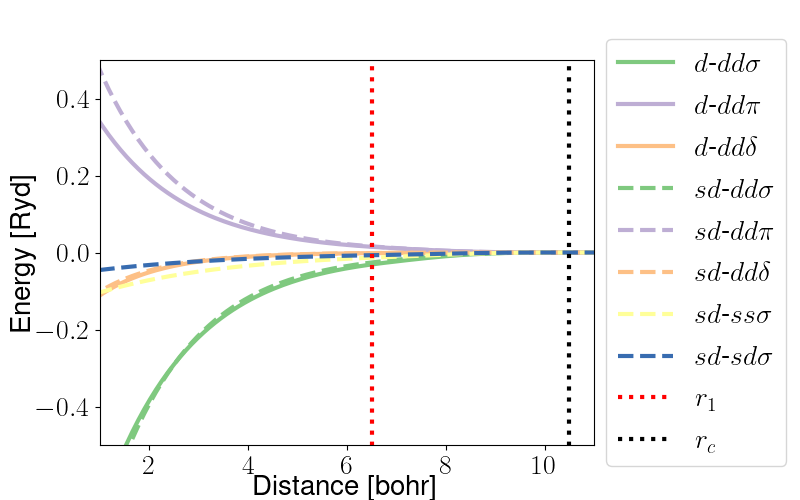
\includegraphics[width=\textwidth]{pictures/sd-d_bond_integrals_together.png}
    \caption[Bond integrals of both $d$ and $sd$ titanium tight-binding models.] {Bond integrals of both $d$ and $sd$ titanium tight-binding models. First and second derivatives shown to demonstrate that there are no abberations when the bond integrals decay to zero between $r_1$ and $r_c$.} %square is table contents, curly is in the chapter
    \label{fig:d_sd_bond_integrals}
  \end{center}
\end{figure}

The bond integrals and pair potential were fitted to reproduce DFT
and empirical data, as detailed in table \textbf{INSERT TABLE REF}.
A loss function was defined as

\begin{equation}
  E(\mathbf{x}) = \sum_i
  w_i(f_i(\mathbf{x}) - \hat{f}_i (\mathbf{x}))^2 + \left[   \alpha
  ||\mathbf{x}||_2 + (1-\alpha) || \mathbf{x} ||_1 \right],
  \label{eq:loss_function}
\end{equation}
where \(\mathbf{x}\) is a vector of input parameters, \(f_i(\mathbf{x})\) are quantities calculated from the
input parameters and \(\hat{f}_i(\mathbf{x})\) are the respective target quantities
from DFT or empirical data. \(w_i\) are the weights for each
quantity. Quantities of higher importance, such as lattice and
elastic constants, were given larger weights in the objective
function, as such, the optimiser would have a preference to
minimise these quantities. To mitigate the overfitting of
parameters (and to dissuade parameters from becoming too large), an Elastic Net regularisation
term was added to the loss function, the final term in equation
\eqref{eq:loss_function}, which consists of the L1 and L2 of the
input parameter vector \(\mathbf{x}\). The L2 norm acts as a penalty
for large input parameters, and the L1 norm also
gives penalties with the added benefit of allowing sparsity of the
parameters: it allows redundant parameters, say in the pair
potential, to go to zero \cite{Hastie2009,Bishop2006}.

The objective function was minimised within pre-defined constraints by use of the the CMA-ES
(Covariance Matrix Adaptation-Evolution Strategy) algorithm by use
of the python implementation by Hansen
\cite{hansen2019pycma}. Parameters put into the CMA-ES
algorithm were first transformed to have similar sensitivities
with respect to the bounds in which they are sought \cite{Hansen2016}. This
allows for the initial assumption of the CMA-ES algorithm, that the
covariance matrix is unity, to be more well satsified, allowing
for a more even traversal of the parameter space
\cite{Jastrebski2006}. Parameters were consequently transformed back,
allowing for evaluation of the objective function and
loss function, of which the latter was consequently fed into the CMA-ES optimiser.


The data used to fit to was a mix of DFT and empirical data. Great
importance was given to the hcp lattice parameter, and the
structural energy differences between the titanium polymorphs, all
of which were compared to GGA LMTO calculations using the questaal
suite \cite{Pashov2020}. Bandwidths at the high symmetry points of
the hcp bands were used as targets, and calculated from DFT by
ascertaining bands of dominant \(d\) character and taking the
difference between the highest and lowest eigenvalues. \(d\)
character was determined by by decomposition of the eigenvector
norm by summation over corresponding orbital subsets, similar to a
Mulliken analysis.

To hasten the fitting of parameters, if a set of parameters
produced a quantity which was out of an acceptable range, then the
objective function would immediately cease and submit a large value
to the objective function, dissuading the optimisation algorithm
from searching around that area in parameter space.

Results from the first stages of fitting found that
soft modes would appear in the phonon spectra for omega and hcp
phases. As such it was necessary to calculate the phonon density of
states in the objective function, to check that there are no
negative densities, as represented in the \texttt{phonopy} code
\cite{Togo2015}  \unit{\milli\gram\per\hour}.

The parameters obtained are shown in table \ref{table:titanium_objective_function}

\begin{table}[H]
  \centering
  \begin{tabular}{lccc}
     Quantity  &    $d$ model &   $sd$ model &       Target \\
     \hline
    $a_{\text{hcp}}$ [\unit{\bohr}]&   5.585 &   5.674 &   5.577 \\
    $c/a(\text{hcp})$ &   1.584 &   1.586 &   1.587 \\
     $a_{\text{omega}}$ [\unit{\bohr}] &   8.935 &   9.039 &   8.733 \\
     $c_{\text{omega}}$ [\unit{\bohr}] &   5.387 &   5.486 &   5.323 \\
     $a_{\text{4h}}   $ [\unit{\bohr}] &   5.576 &   5.681 &   5.563 \\
     $c_{\text{4h}}   $ [\unit{\bohr}] &  18.098 &  18.328 &  17.759 \\
     $a_{\text{6h}}   $ [\unit{\bohr}] &   5.574 &   5.676 &   5.546 \\
     $c_{\text{6h}}   $ [\unit{\bohr}] &  27.184 &  27.579 &  26.771 \\
     $a_{\text{bcc}}  $ [\unit{\bohr}] &   6.201 &   6.201 &   6.179 \\
    $a_{\text{fcc}}  $ [\unit{\bohr}] &   7.873 &   8.013 &   7.887 \\
    \hline
     $E(\omega) - E( \text{hcp})  [\unit{\milli\rydberg}]$ &   0.588 &  -0.357 &  -0.633 \\
     $E(4h)- E(\text{hcp}) $ [\unit{\milli\rydberg}] &   1.580 &   1.663 &   3.172 \\
     $E(6h)- E(\text{hcp}) $ [\unit{\milli\rydberg}] &   2.483 &   2.400 &   3.720 \\
     $E(\text{bcc}) - E( \text{hcp})  $ [\unit{\milli\rydberg}] &   5.351 &   7.958 &   7.635 \\
     $E(\text{fcc}) - E( \text{hcp})  $ [\unit{\milli\rydberg}] &   3.780 &   3.825 &   4.519 \\
    \hline
     $C_{11}$ [\unit{\GPa}] & 171.6 & 167.3 & 176.1 \\
     $C_{33}$ [\unit{\GPa}] & 198.9 & 205.2 & 190.5 \\
     $C_{44}$ [\unit{\GPa}] &  47.4 &  46.6 &  50.8 \\
     $C_{12}$ [\unit{\GPa}] &  94.7 &  96.7 &  86.9 \\
     $C_{13}$ [\unit{\GPa}] &  61.2 &  60.9 &  68.3 \\
    \hline
    hcp bandwidth $\Gamma$ [$\unit{\eV}$] &   3.69 &   8.90 &   5.87 \\
    hcp bandwidth $K$ [\unit{\eV}] &   4.65 &   4.79 &   4.97 \\
    hcp bandwidth $M$ [\unit{\eV}] &   5.19 &   5.54 &   7.78 \\
    hcp bandwidth $L$ [\unit{\eV}] &   4.21 &   5.43 &   6.34 \\
    hcp bandwidth $H$ [\unit{\eV}] &   3.54 &   4.85 &   9.70 \\
    \hline
    $E_{\text{prismatic}$ fault  &         99.0 &        110.4 & 220.0 \\
    $E_{\text{basal}$ fault &              &        208.9 &              \\
    $E_{\text{pyramidal I}$ fault   &              &        154.6 &              \\

  \end{tabular}
  \caption[Table of the titanium objective function values compared to DFT target data.] {Table of the titanium objective function values compared to DFT target data. The hcp lattice parameter, and the structural energy differences between titanium polymorphs were given large weights in the objective function. \label{table:titanium_objective_function}}
  \end{table}





----------     E\textsubscript{prismatic}\textsubscript{fault}     -----------

\begin{center}
\begin{tabular}{lrll}
tbe: & 98.953 & mJ/m\textsuperscript{2} & \\
DFT: & 250.000 & mJ/m\textsuperscript{2} & [Benoit  2012]\\
DFT: & 233.000 & mJ/m\textsuperscript{2} & [Ackland 1999]\\
\end{tabular}
\end{center}


----------     E\textsubscript{Basal}\textsubscript{fault} I2     -----------

\begin{center}
\begin{tabular}{lrll}
tbe: & 211.658 & mJ/m\textsuperscript{2} & \\
DFT: & 260.000 & mJ/m\textsuperscript{2} & [Benoit  2012]\\
\end{tabular}
\end{center}

\subsection{sd fitting: Including hybridisation}
\label{sec:orgc242e48}

We included s orbitals such that one could more readily model the
Ti\(^{4+}\) oxidation state of the Ti ion, which would give a more
physical representation of titanium ions in quantum electrochemistry
calculations.
\end{document}